\section{Model Exercise 0-1b (01): Bending fracture test (OPA)}
\label{sec:mex01b}
\Authors{Amir Sattari, Keita Yoshioka}

\subsection{Experimental set-up and results}

In addition, the effect of the anisotropy on the fracture toughness of the Opalinus claystones experimentally and numerically is investigated. The description of the experimental setup and the test procedure is explained in section \ref{sec:Fracture_Toughness_Exp}, where a fracture toughness test on a sample with the dimension of $140Lx30Wx30T (mm)$ is carried out. The notch dimension is $2LX10Wx30T (mm)$ and the span length ($s$) is $120 mm$. The anisotropy of a claystone depends mainly on the orientation of the embedded layers. When the loading direction is perpendicular ($\bot$) to the layering orientation the materials strength is highest. In contrast, when the loading direction is parallel ($\parallel$) to the layering orientation, the materials strength is the lowest. The peak load attained from the experimental data ($\bot$) is $598 N$ and the bending stiffness ($E_b$) is around $3.3 GPa$. The crack mouth opening before the failure is $24 \mu m$. The 4K video with the 30fps is used to track the reference points on the claystone. Afterward, the image analyzing technique is implemented to determine the CMOD. The 30fps video was not enough to detect the brittle failure of the sample and therefore in the experimental data, the post failure response is not well represented. The measured fracture toughness ($\bot$) is $0.746\ MPa.\sqrt\ m$.

\subsection{Model approach}

\subsubsection*{Lattice-Element-Model (LEM)}

The LEM is implemented to investigate the anisotropy of claystone in two cases, where the loading direction is parallel or perpendicular to the layering orientation. The LEM setup ($\bot$) is generated in 2D with the back calculation of the input data from the experimental results from fracture toughness (sec. \ref{sec:Fracture_Toughness_Exp}) and splitting (sec. \ref{sec:Brazilian_Disk_Exp}) tests. The materials strength in perpendicular direction is considered to be 5 times higher than parallel case. The fracture paths for both ($\bot$) and ($\parallel$) cases are shown in \ref{fig:Amir_ME1_LEM_Perpendicular} and \ref{fig:Amir_ME1_LEM_Parallel}, respectively. \ref{fig:Amir_ME1_LEM_Claystone} illustrates the comparison between the experimental and numerical data. As discussed before, the post failure behavior does not match due to the experimental shortage of capturing the true load-displacements.

\begin{figure}[!ht]
\centering
\begin{subfigure}[b]{0.55\textwidth}
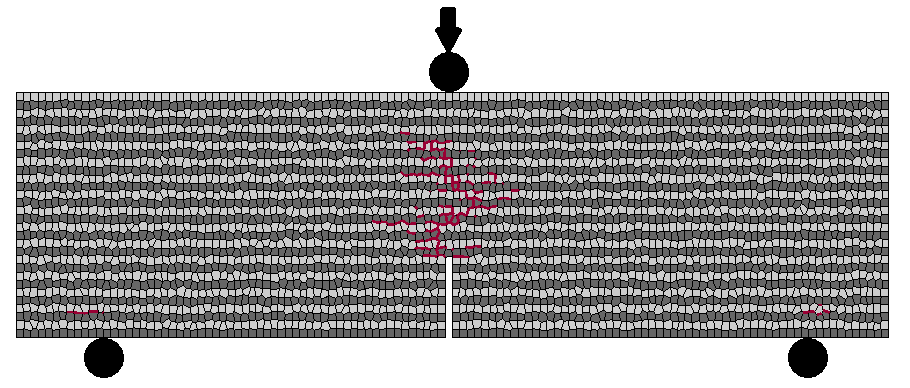
\includegraphics[width=1\linewidth]{figures/Amir_ME1_LEM_Perpendicular.png}
\subcaption{}
\label{fig:Amir_ME1_LEM_Perpendicular}
\end{subfigure}
%\hfill
\begin{subfigure}[b]{0.55\textwidth}
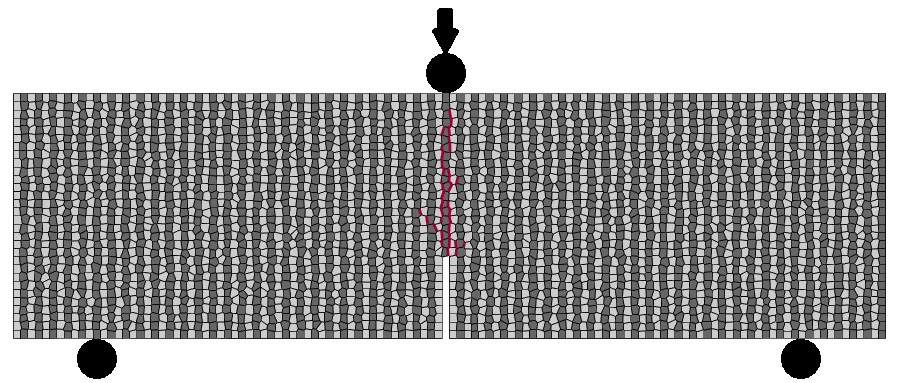
\includegraphics[width=1\linewidth]{figures/Amir_ME1_LEM_Parallel.png}
\subcaption{}
\label{fig:Amir_ME1_LEM_Parallel}
\end{subfigure}
\caption{The fracking path under condition of loading direction (a) perpendicular, and (b) parallel to the layering orientation}
\end{figure}

\begin{figure}[!ht]
\centering
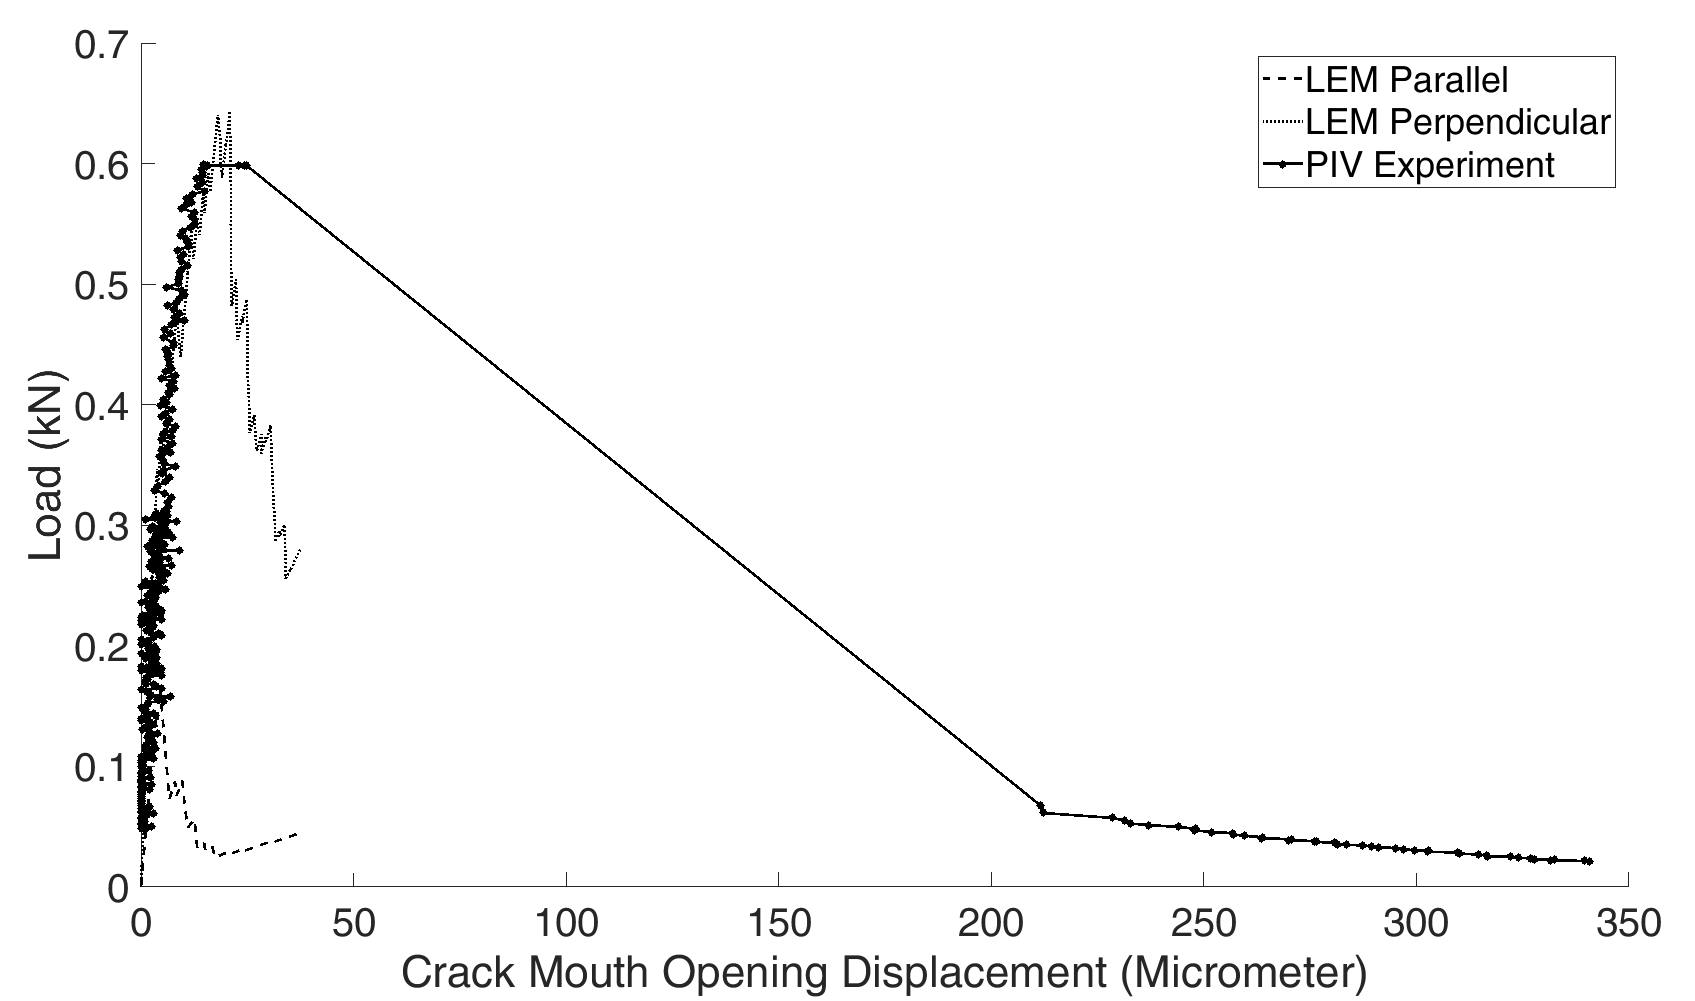
\includegraphics[width=0.75\textwidth]{figures/Amir_ME1_LEM_Claystone.png}
\caption{The comparison of experimental and numerical data for effect of anisotropy in Opalinus claystone} 
\label{fig:Amir_ME1_LEM_Claystone}
\end{figure}

\subsubsection*{Finite-Element-Approach: Variational Phase-Field (VPF)}

Extended experiment: parallel to the lamination Fig.~\ref{fig:ME1_ext_vpf_para_init} and orthogonal to the lamination Fig.~\ref{fig:ME1_ext_vpf_orth_init}.
Fracture simulation results are in Figs.~\ref{fig:ME1_ext_vpf_para_result} and~\ref{fig:ME1_ext_vpf_orth_result}, and the force vs. CMOD is in Fig~\ref{fig:ME1_ext_vpf_FvsCMOD}.

\begin{figure}[!ht]
\centering
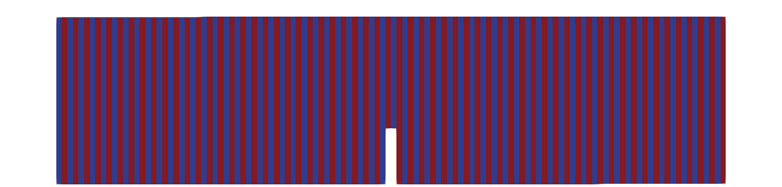
\includegraphics[width=1\textwidth]{figures/ME1_ext_2D_parallel_init.png}
\caption{Sample for parallel to the lamination}
\label{fig:ME1_ext_vpf_para_init}
\end{figure}

\begin{figure}[!ht]
\centering
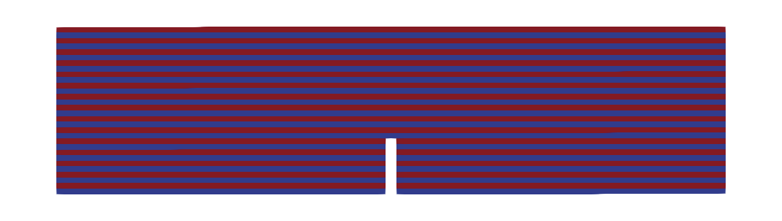
\includegraphics[width=1\textwidth]{figures/ME1_ext_2D_orthogonal_init.png}
\caption{Sample for orthogonal to the lamination}
\label{fig:ME1_ext_vpf_orth_init}
\end{figure}

\begin{figure}[!ht]
\centering
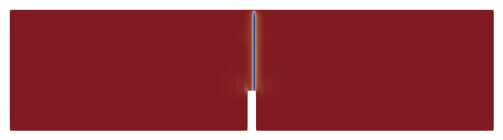
\includegraphics[width=1\textwidth]{figures/ME1_ext_2D_para_result.png}
\caption{Result of parallel to the lamination}
\label{fig:ME1_ext_vpf_para_result}
\end{figure}

\begin{figure}[!ht]
\centering
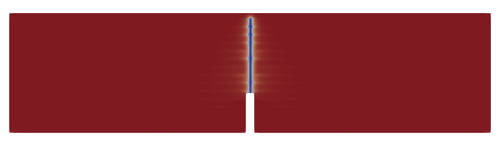
\includegraphics[width=1\textwidth]{figures/ME1_ext_2D_orth_result.png}
\caption{Result of orthogonal to the lamination}
\label{fig:ME1_ext_vpf_orth_result}
\end{figure}

\begin{figure}[!ht]
\centering
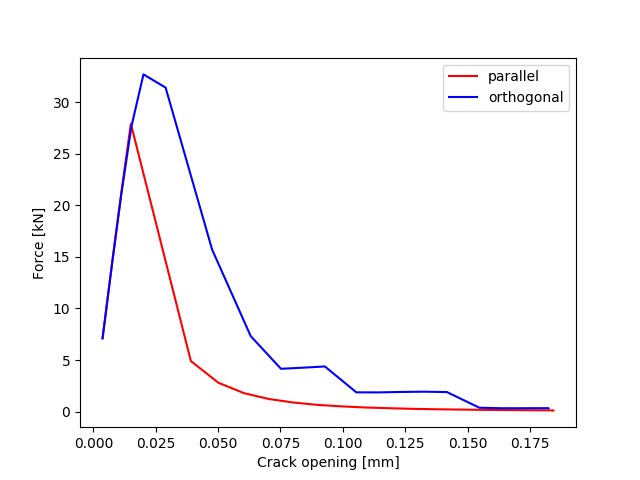
\includegraphics[width=1\textwidth]{figures/ME1_ext_NFvsCMOD.png}
\caption{Force vs. CMOD}
\label{fig:ME1_ext_vpf_FvsCMOD}
\end{figure}

\todo[inline]{[UFZ](KY): Description of OGS-VPF results}

\subsubsection{Results and discussion}

\todo[inline]{[CAU/UFZ](AS/KY): Short comparison of results}